% \section{Method Lookup Algorithm and Auxiliary Definitions}\label{sec:auxdefs}
\section{Key Algorithms and Type-Soundness}\label{sec:auxdefs}
In this section, we present the fundamental algorithms and auxiliary
definitions used in our formalization, and show that the resulting
calculus is type sound. The functions presented in this section are
the key components that implement our algorithm for method lookup.

\subsection{Method Lookup Algorithm in \mbody{}}\label{subsec:mbodydef}

$\mbody(m, I_d, I_s)$ denotes the method body lookup function.
We use $I_d, I_s$, since $\mbody$ is usually invoked by a receiver of a method $m$, with its dynamic type $I_d$ and static type $I_s$. Such a function returns the most specific method implementation. More
accurately, $\mbody$ returns the parameters, returned expression
(empty for abstract methods) and the types for the method. It considers both originally-defined methods and hierarchical overriding methods, so $\mostSpecific$ and $\mostSpecificOverride$ (see the definition in Section~\ref{sec:mostSpecific} and Section~\ref{sec:mostSpecificOverride}) are both invoked.
 The formal definition gives the expected results
for the earlier examples in Figure~\ref{fig:examplesmbody}.

\begin{flalign*}
	& \rhd \textit{Definition of } \mbody(m, I_d, I_s): & \\
	& \bullet \mbody(m, I_d, I_s) = (J, \overline{I_x} \; \overline{x}, I_e \; e_0) & \\
	& \indent\indent \textrm{with: } \mostSpecific(m, I_d, I_s) = \{I\} & \\
	& \hspace{.77in} \mostSpecificOverride(m, I_d, I) = \{J\} & \\
	& \hspace{.77in} J[m\ \kwoverride\ I] = \method{I_e}{m}{I_x}{x}{I}{e_0} & \\
	& \bullet \mbody(m, I_d, I_s) = (J, \overline{I_x} \; \overline{x}, I_e \; \o) & \\
	& \indent\indent \textrm{with: } \mostSpecific(m, I_d, I_s) = \{I\} & \\
	& \hspace{.77in} \mostSpecificOverride(m, I_d, I) = \{J\} & \\
	& \hspace{.77in} J[m\ \kwoverride\ I] = \absmethod{I_e}{m}{I_x}{x}{I} & \\
\end{flalign*}
To calculate $\mbody(m, I_d, I_s)$, the invocation of $\mostSpecific$ looks for the most specific original methods and their interfaces, and expects a singleton set, so as to avoid unambiguity. Furthermore, the invocation of $\mostSpecificOverride$ also expects a unique (unambiguous) most specific hierarchical override. And finally the target method is returned.

\subsection{Finding the Most Specific Origin: \mostSpecific}\label{sec:mostSpecific}
\haoyuan{Visualize findorigin and findoverride with some figures.}
We proceed to give the definitions of two core functions that support method lookup, namely \mostSpecific{} and \mostSpecificOverride. Generally,
$\mostSpecific(m, I, J)$ finds the set of most specific interfaces where $m$ is originally defined. As shown in Figure~\ref{fig:findOrigin}(left), interfaces in this set should be above interface $I$ and along path $J$. ``Along path $J$'' means the interface should be either a subtype or a super type of $J$, visually, it should locate between $J$ and $I$ or above $J$. Finally with $\prune$ (defined in Section~\ref{sec:otherdefs})
the overridden interfaces will be filtered out.

\begin{flalign*}
	& \rhd \textit{Definition of } \mostSpecific(m, I, J): & \\
	& \bullet \mostSpecific(m, I, J) = \prune(origins) & \\
	& \indent\indent \textrm{with: } origins = \{K \mid \subt{I}{K}, \textrm{ and } \subt{K}{J} \; \lor \; \subt{J}{K}, &\\
	& \hspace{1.62in} \textrm{ and } K[m\ \kwoverride\ K] \textrm{ is defined} \} &
\end{flalign*}
By the definition, an interface belongs to $\mostSpecific(m, I, J)$ if and only if:
\begin{itemize}
	\item It originally defines $m$;
	\item It is a super type of $I$;
	\item It is either a super type or a subtype of $J$ (including $J$ itself);
	\item Any subtype of it does not belong to the same result set because of $\prune$.
\end{itemize}

\begin{figure*}[t]
  % \nocaptionrule
  % \centering
  \centering
  \begin{minipage}[t]{0.55\textwidth}
  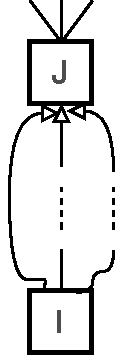
\includegraphics[width=1cm]{pics/P10.pdf}
  \end{minipage}
  \centering
  \hspace*{2pt}
  \begin{minipage}[t]{0.35\textwidth}
  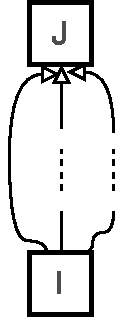
\includegraphics[width=1cm]{pics/P9.pdf}
  \end{minipage}  
  \caption{UMLs illustrating \mostSpecific(left) and \mostSpecificOverride(right)}\label{fig:findOrigin}
\end{figure*}


\subsection{Finding the Most Specific Overriding: \mostSpecificOverride}\label{sec:mostSpecificOverride}
The $\mostSpecific$ function only focuses on original method
implementations, all the hierarchical overriding methods are omitted
during that step. On the other hand, $\mostSpecificOverride(m, I, J)$
has the assumption that $J$ defines an original $m$, and this function
tries to find the interfaces with the most specific implementations that hierarchically overrides such an $m$. Formally,

\begin{flalign*}
	& \rhd \textit{Definition of } \mostSpecificOverride(m, I, J): & \\
	& \bullet \mostSpecificOverride(m, I, J) = \prune(overrides) & \\
	& \indent\indent \textrm{with: } overrides = \{K \mid \subt{I}{K}, \; \subt{K}{J} \textrm{ and } K[m\ \kwoverride\ J] \textrm{ is defined} &
\end{flalign*}
By the definition, as shown in Figure~\ref{fig:findOrigin}, an interface belongs to $\mostSpecific(m, I, J)$ if and only if:
\begin{itemize}
	\item it is between $I$ and $J$;
	\item it hierarchically overrides $J.m$;
	\item any subtype of it does not belong to the same set.
\end{itemize}


\subsection{Other Auxiliaries}\label{sec:otherdefs}
Below we give other minor definitions of the auxiliary functions that are used in previous sections.

%%%%============================ I[m override J] ================%%%%%%%%
\begin{flalign*}
	& \rhd \textit{Definition of } I[m\ \kwoverride\ J]: & \\
	& \bullet I[m\ \kwoverride\ J] = \method{I_e}{m}{I_x}{x}{J}{e_0} & \\
	& \indent\indent \textrm{with: }
	  \kwinterface \; I \; \kwextends \; \overline{I} \; \{ \method{I_e}{m}{I_x}{x}{J}{e_0} \ldots \} & \\
	& \bullet I[m\ \kwoverride\ J] = \absmethod{I_e}{m}{I_x}{x}{J} & \\
	& \indent\indent \textrm{with: }
	\kwinterface \; I \; \kwextends \; \overline{I} \; \{ \absmethod{I_e}{m}{I_x}{x}{J} \ldots \} & \\
\end{flalign*}
Here $I[m\ \kwoverride\ J]$ is basically a direct lookup for method $m$ in the body of $I$, where such a method
overrides $J$ (like static dispatch). The method can be either concrete or abstract, and the body of definition is returned. Notice that
by our syntax, $I[m\ \kwoverride\ I]$ is looking for the originally-defined method $m$ in $I$.
%%%%============================ I[m override J] end================%%%%%%%%

%%%%============================ prune(set) ================%%%%%%%%
\begin{flalign*}
	& \rhd \textit{Definition of } \prune(set): & \\
	& \bullet \prune(set) = \{I \in set \; | \; \nexists J \in set\setminus I, J <: I\} &
\end{flalign*}
The $\prune$ function takes a set of
types, and filters out those that have subtypes in the same set. In the returned set,
none of them has subtyping relation to one another, since all super types have been removed.
%%%%============================ prune(set) end ================%%%%%%%%

%%%%============================ canOverride ================%%%%%%%%
\begin{flalign*}
	& \rhd \textit{Definition of } \canOverride(m, I, J): & \\
	& \bullet \canOverride(m, I, J) = True & \\
	& \indent\indent \textrm{with: } I[m\ \kwoverride\ I] = I_e \; m(\overline{I_x} \; \overline{x}) \; \kwoverride \; I \ldots & \\
	& \hspace{.77in} J[m\ \kwoverride\ J] = I_e \; m(\overline{I_x} \; \overline{y}) \; \kwoverride \; J \ldots &
\end{flalign*}
$\canOverride$ just checks that two original $m$ in $I$ and $J$ have the same type.
%%%%============================ canOverride end ================%%%%%%%%

%%%%============================ canInstantiate ================%%%%%%%%
\begin{flalign*}
	& \rhd \textit{Definition of } \canInstantiate(I): & \\
	& \bullet \canInstantiate(I) = True & \\
	& \indent\indent \textrm{with: } \forall m, \forall J \in \mostSpecific(m, I, I), \mostSpecificOverride(m, I, J) = \{K\}, & \\
	& \hspace{.77in} \textrm{ and } K[m\ \kwoverride\ J] = \method{I_e}{m}{I_x}{x}{J}{e_0} &
\end{flalign*}
$\canInstantiate(I)$ checks whether interface $I$ can be instantiated by the keyword $\kwnew$.
$\mostSpecific(m, I, I)$ represents the set of branches $I$ inherits on method $m$. $I$ can be instantiated
if and only if for every branch, the most specific implementation is unambiguous and non-abstract.
%%%%============================ canInstantiate end ================%%%%%%%%

\subsection{Properties}

We present the type soundness of the model by a few theorems below, following the standard technique of
subject reduction and progress proposed by Wright and Felleisen~\cite{Wright1994}. The proof, together with some lemmas, are
in Appendix. Type soundness states that if an expression is well-typed, then after many reduction
steps it must reduce to a value, and its annotation is the same as the static type of the original expression.

\begin{theorem}[Subject Reduction]~\label{theorem_subject}
If $\judgeewf \Gamma {e : I}$ and $e \rightarrow e'$, 
then $\judgeewf \Gamma {e' : I}$.
\end{theorem}
\begin{proof}
See Appendix~\ref{appendix_proof}.
\end{proof}

\begin{theorem}[Progress]~\label{theorem_progress}
Suppose $e$ is a well-typed expression, if $e$ includes 
$\left((J)\emph{\kwnew}\;I()\right).m(\overline{v})$ as a sub-expression, then $\mbody(m, I, J) = (I_0, \overline{I_x} \; \overline{x}, I_e\; e_0)$ and $\num{\overline{x}} = \num{\overline{v}}$ for some $I_0$, $\overline{I_x}$, $\overline{x}$, $I_e$ and $e_0$.
\end{theorem}
\begin{proof}
See Appendix~\ref{appendix_proof}.
\end{proof}

\begin{theorem}[Type Soundness]~\label{theorem_soundness}
If $\judgeewf \o {e : I}$ and $e \to^* e'$ with $e'$ a normal form, then $e'$ is 
a value $v$ with $\judgeewf \o {v:I}$.
\end{theorem}
\begin{proof}
Immediate from Theorem~\ref{theorem_subject} and Theorem~\ref{theorem_progress}.
\end{proof}
Note that in Theorem~\ref{theorem_progress}, ``$\#(\overline{x})$'' denotes the length of
$\overline{x}$.

Our theorems are stricter than those of Featherweight Java~\cite{Igarashi01FJ}. Specifically, in both term substitution (a lemma in Appendix)
and subject reduction, reduction may lead to a term with a subtype in
FJ, but in \MIM{} types are unchanged. The difference is due to
%%subtyping; the parameter or \lstinline|this| reference requires some type $I$, but a value with a more specific type,
%%which is subtype of $I$, can be passed. However, as 
the fact that \MIM{} keeps track of the static types during
reduction. 
In FJ, the information about the static types is lost. 

%the annotations in the
%substitution actually ensures the type to be unchanged.